\documentclass[a4paper,landscape,9pt]{article}

\usepackage[margin=1cm]{geometry}
\usepackage{fontspec}
\setmainfont{TeX Gyre Pagella}
\usepackage{unicode-math}
\setmathfont{TeX Gyre Pagella Math}

\usepackage{tikz}
\usetikzlibrary{arrows.meta,calc,positioning,shapes.geometric}
\usepackage{microtype}

\pagestyle{empty}
\setlength{\parindent}{0pt}
\setlength{\parskip}{0.25em}

\tikzset{
  node-d/.style={draw,fill=black,regular polygon,regular polygon sides=6,minimum size=7mm,inner sep=0pt,text=white,font=\tiny\bfseries},
  node-a/.style={draw,fill=black!70,regular polygon,regular polygon sides=3,minimum size=7mm,inner sep=0pt,text=white,font=\tiny\bfseries},
  node-t/.style={draw,circle,minimum size=7mm,inner sep=0pt,line width=0.4pt,font=\tiny},
  node-o/.style={draw,fill=black!15,rectangle,minimum size=7mm,inner sep=0pt,font=\tiny},
  node-i/.style={draw,diamond,minimum size=8mm,inner sep=0pt,line width=0.4pt,font=\tiny},
  impl/.style={-{Latex[length=1.2mm]},line width=0.3pt,black!80},
  exemp/.style={-{Latex[length=1.2mm]},line width=0.3pt,dashed,black!80},
  band/.style={font=\scriptsize\scshape,text=black!60},
  bandline/.style={draw,black!18,line width=0.3pt},
}

\begin{document}

\begin{center}
{\large\scshape Proposisjonsgraf, seksjon 1}\hspace{0.8em}{\itshape Formverda er alt som er tilfelle}
\end{center}

\vspace{-0.6em}

\begin{center}
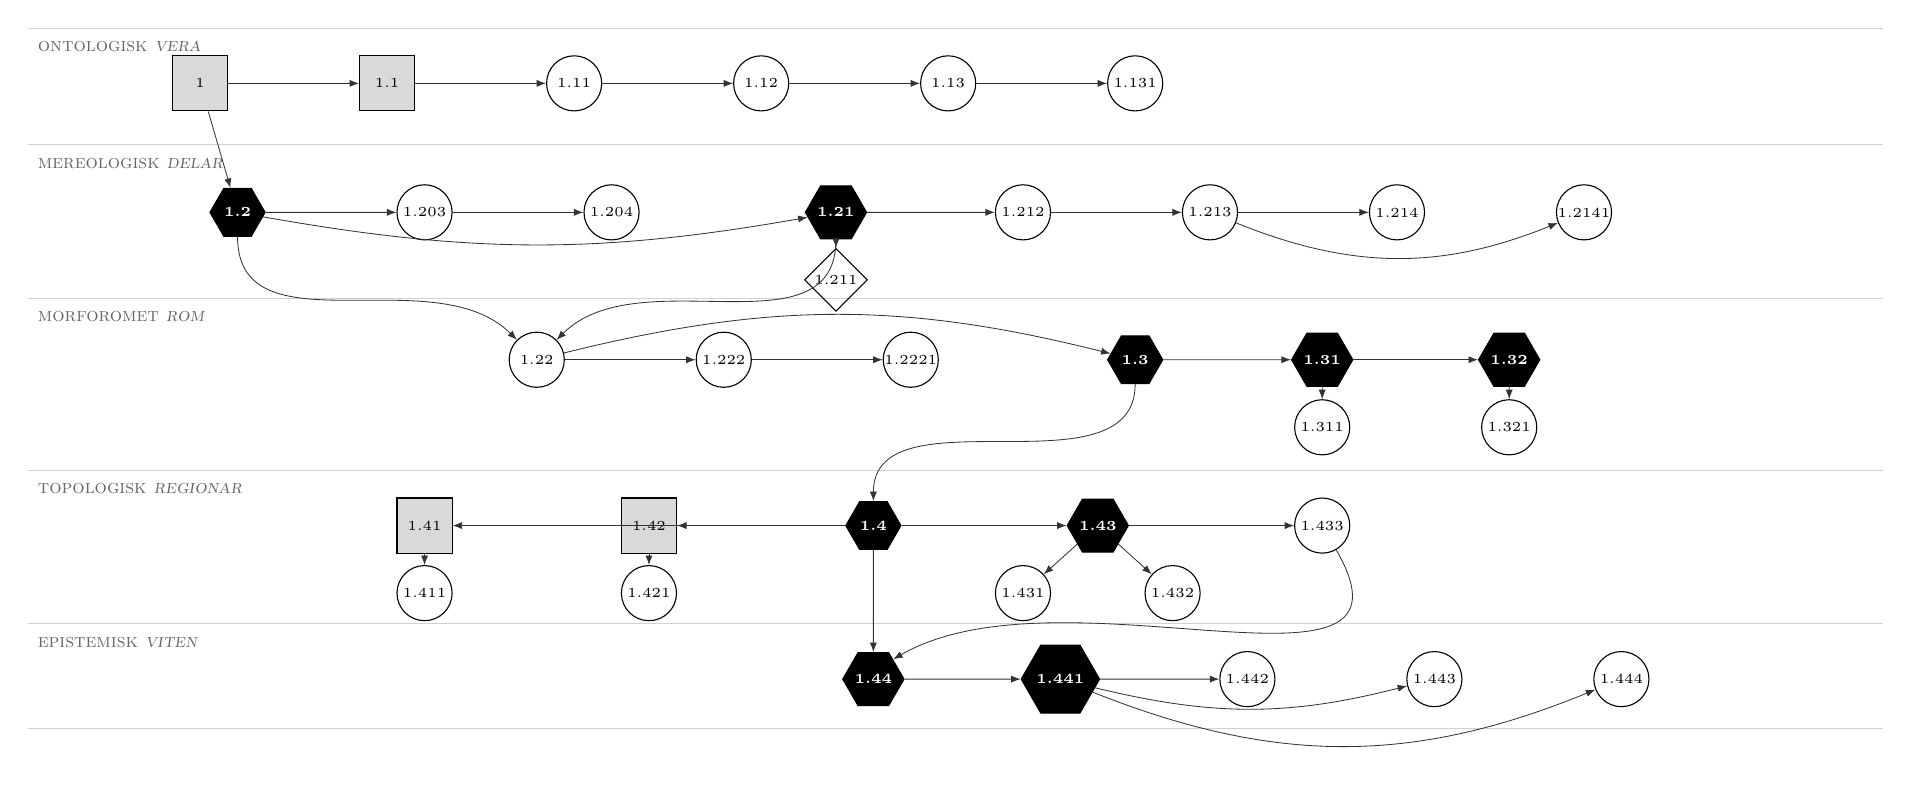
\begin{tikzpicture}[x=0.95cm,y=0.78cm]

  \draw[bandline] (-0.3, 0.6)   -- (24.5, 0.6);
  \draw[bandline] (-0.3, -1.3)  -- (24.5, -1.3);
  \draw[bandline] (-0.3, -3.8)  -- (24.5, -3.8);
  \draw[bandline] (-0.3, -6.6)  -- (24.5, -6.6);
  \draw[bandline] (-0.3, -9.1) -- (24.5, -9.1);
  \draw[bandline] (-0.3, -10.8) -- (24.5, -10.8);

  \node[band,anchor=west] at (-0.3, 0.3)  {ontologisk  \itshape vera};
  \node[band,anchor=west] at (-0.3, -1.6) {mereologisk  \itshape delar};
  \node[band,anchor=west] at (-0.3, -4.1) {morforomet  \itshape rom};
  \node[band,anchor=west] at (-0.3, -6.9) {topologisk  \itshape regionar};
  \node[band,anchor=west] at (-0.3, -9.4) {epistemisk  \itshape viten};

  % BAND 1
  \node[node-o] (p1)     at (2, -0.3)    {1};
  \node[node-o] (p11)    at (4.5, -0.3)  {1.1};
  \node[node-t] (p111)   at (7, -0.3)    {1.11};
  \node[node-t] (p112)   at (9.5, -0.3)  {1.12};
  \node[node-t] (p113)   at (12, -0.3)   {1.13};
  \node[node-t] (p1131)  at (14.5, -0.3) {1.131};
  \draw[impl] (p1) -- (p11);
  \draw[impl] (p11) -- (p111);
  \draw[impl] (p111) -- (p112);
  \draw[impl] (p112) -- (p113);
  \draw[impl] (p113) -- (p1131);

  % BAND 2
  \node[node-d] (p2)     at (2.5, -2.4)  {1.2};
  \node[node-t] (p203)   at (5, -2.4)    {1.203};
  \node[node-t] (p204)   at (7.5, -2.4)  {1.204};
  \node[node-d] (p21)    at (10.5, -2.4) {1.21};
  \node[node-i] (p211)   at (10.5, -3.5) {1.211};
  \node[node-t] (p212)   at (13, -2.4)   {1.212};
  \node[node-t] (p213)   at (15.5, -2.4) {1.213};
  \node[node-t] (p214)   at (18, -2.4)   {1.214};
  \node[node-t] (p2141)  at (20.5, -2.4) {1.2141};
  \draw[impl]  (p1) -- (p2);
  \draw[impl]  (p2) -- (p203);
  \draw[impl]  (p203) -- (p204);
  \draw[impl]  (p2) to[bend right=10] (p21);
  \draw[exemp] (p21) -- (p211);
  \draw[impl]  (p21) -- (p212);
  \draw[impl]  (p212) -- (p213);
  \draw[impl]  (p213) -- (p214);
  \draw[impl]  (p213) to[bend right=22] (p2141);

  % BAND 3
  \node[node-t] (p22)    at (6.5, -4.8)  {1.22};
  \node[node-t] (p222)   at (9, -4.8)    {1.222};
  \node[node-t] (p2221)  at (11.5, -4.8) {1.2221};
  \node[node-d] (p3)     at (14.5, -4.8) {1.3};
  \node[node-d] (p31)    at (17, -4.8)   {1.31};
  \node[node-t] (p311)   at (17, -5.9)   {1.311};
  \node[node-d] (p32)    at (19.5, -4.8) {1.32};
  \node[node-t] (p321)   at (19.5, -5.9) {1.321};
  \draw[impl] (p2) to[out=-90,in=135] (p22);
  \draw[impl] (p21) to[out=-90,in=45] (p22);
  \draw[impl] (p22) -- (p222);
  \draw[impl] (p222) -- (p2221);
  \draw[impl] (p22) to[bend left=14] (p3);
  \draw[impl] (p3) -- (p31);
  \draw[impl] (p31) -- (p311);
  \draw[impl] (p31) -- (p32);
  \draw[impl] (p32) -- (p321);

  % BAND 4
  \node[node-d] (p4)     at (11, -7.5)   {1.4};
  \node[node-o] (p41)    at (5, -7.5)    {1.41};
  \node[node-t] (p411)   at (5, -8.6)    {1.411};
  \node[node-o] (p42)    at (8, -7.5)    {1.42};
  \node[node-t] (p421)   at (8, -8.6)    {1.421};
  \node[node-d] (p43)    at (14, -7.5)   {1.43};
  \node[node-t] (p431)   at (13, -8.6)   {1.431};
  \node[node-t] (p432)   at (15, -8.6)   {1.432};
  \node[node-t] (p433)   at (17, -7.5)   {1.433};
  \draw[impl] (p3) to[out=-90,in=90] (p4);
  \draw[impl] (p4) -- (p41);
  \draw[impl] (p4) -- (p42);
  \draw[impl] (p4) -- (p43);
  \draw[impl] (p41) -- (p411);
  \draw[impl] (p42) -- (p421);
  \draw[impl] (p43) -- (p431);
  \draw[impl] (p43) -- (p432);
  \draw[impl] (p43) -- (p433);

  % BAND 5
  \node[node-d] (p44)    at (11, -10)    {1.44};
  \node[node-d] (p441)   at (13.5, -10)  {1.441};
  \node[node-t] (p442)   at (16, -10)    {1.442};
  \node[node-t] (p443)   at (18.5, -10)  {1.443};
  \node[node-t] (p444)   at (21, -10)    {1.444};
  \draw[impl] (p4) -- (p44);
  \draw[impl] (p433) to[out=-60,in=30,looseness=1.1] (p44.north east);
  \draw[impl] (p44) -- (p441);
  \draw[impl] (p441) -- (p442);
  \draw[impl] (p441) to[bend right=14] (p443);
  \draw[impl] (p441) to[bend right=22] (p444);

\end{tikzpicture}
\end{center}

\vspace{-0.2em}

\hrule

\vspace{0.4em}

\begin{minipage}[t]{0.325\textwidth}
{\scshape\small Lesing ovanfrå}

Grafen har éi rot og fem epistemiske band. Rota er proposisjon \emph{1}: \emph{formverda er alt som er tilfelle}. Alt som følgjer, kviler på henne.

Frå rota greinar seg ein ontologisk kjede horisontalt gjennom band 1, og ein mereologisk kaskade ned til band 2. Band 2 deler seg straks i to parallelle spor: objektet (\emph{1.2}) og konfigurasjonen (\emph{1.21}). Desse to møtest i \emph{1.22}, som er seksjonens einaste ekte syntese.
\end{minipage}\hfill
\begin{minipage}[t]{0.325\textwidth}
{\scshape\small Lesing nedover}

Frå \emph{1.22} veks morforomet fram som eksplisitt definisjon (\emph{1.3}). Projeksjonsomgrepet (\emph{1.32}) står som hjørnestein for alt empirisk arbeid seinare.

Frå \emph{1.3} stig den topologiske partisjonen (\emph{1.4}) og deler seg i tre regionar: busett (\emph{1.41}), open (\emph{1.42}), forboden (\emph{1.43}). \emph{1.433} er ein hengsel; han seier at topologi og epistemologi ikkje er same sak, og er difor den einaste noden som sender ei pil på tvers av bandgrensa ned til \emph{1.44}.
\end{minipage}\hfill
\begin{minipage}[t]{0.325\textwidth}
{\scshape\small Strukturelle innsikter}

\emph{Konfluens.} \emph{1.22} har to foreldre; alle andre nodar har éin. Dette er seksjonens einaste syntese.

\emph{Definisjonsstige.} Band 2 til 5 startar kvar med ein definisjon (svart sekskant). Band 1 har ingen. Rota er ei rein observasjon, slik det seg hør for ein aksiomatisk tekst.

\emph{Ingen postulat.} Seksjon 1 inneheld ingen triangel. Postulata kjem fyrst i seksjon 2 når seleksjonstrykka skal innførast.

\emph{Ingen ekvivalens.} Ingen dobbel pil her. Reduksjonsteoremet skjer seinare, mellom grammatikk og landskap.
\end{minipage}

\end{document}
